\documentclass[a4paper,12pt]{book}
\usepackage[utf8]{inputenc}
\title{}
\author{Rachel Morris}
\date{\today}

\usepackage{rachwidgets}
\usepackage{fancyhdr}
\usepackage{lastpage}
\usepackage{dirtree}
\usepackage{boxedminipage}
\usepackage{colortbl} % cell bg colors

\setcounter{chapter}{4}
\setcounter{section}{4}
\newcommand{\laChapter}{4.5 Equivalence Relations\ }
\newcounter{question}

\newcommand{\laClass}{CS 210\ }
\newcommand{\laSemester}{Fall 2017\ }

\pagestyle{fancy}
\fancyhf{}
\lhead{\laClass \laSemester}
\chead{}
\rhead{Ch \laChapter}
\rfoot{\thepage\ of \pageref{LastPage}}
\lfoot{\scriptsize Compiled by Rachel Morris, last updated \today}

\renewcommand{\headrulewidth}{2pt}
\renewcommand{\footrulewidth}{1pt}

\begin{document}

    \toggletrue{answerkey}
    \togglefalse{answerkey}

    %------------------------------------------------------------------%
    %- Exercise Begin -------------------------------------------------%
    %------------------------------------------------------------------%

    \section{Equivalence Relations}

    \subsection{Thinking about equivalence}
    
    % -------------------------------------------------------------%
    % - QUESTION --------------------------------------------------%
    % -------------------------------------------------------------%
    \stepcounter{question}
    \begin{questionNOGRADE}{\thequestion}
        
        A person is flipping three coins, and the score that they receive
        is the sum of all the coins together, where Heads = 1, and Tails = 0.
        The minimum point value is 0 (T-T-T), and the maximum is 3 (H-H-H).
        List out all cooin combinations that give equivalent scores.
        Assume coin toss order does matter, so (T-H-H), (H-T-H), and (H-H-T)
        will all be separate outcomes.
        \begin{center}
            \includegraphics{images/coins.png}
        \end{center}
        
        \Large
        \begin{tabular}{c | p{10cm}}
            Points & Coin combinations
            \\ \hline
            0 & \solution{(T-T-T)}{}
            \\ \hline
            1 & \solution{(H-T-T), (T-H-T), (T-T-H)}{}
            \\ \hline
            2 & \solution{(T-H-H), (H-T-H), (H-H-T)}{}
            \\ \hline
            3 & \solution{(H-H-H)}{}
        \end{tabular}
        \normalsize
        ~\\~\\
        \begin{itemize}
            \item[a.]   How many ways are there to get 0 points?    \solution{ 1 }{ ~\\ }
            \item[b.]   How many ways are there to get 1 point?     \solution{ 3 }{ ~\\ }
            \item[c.]   How many ways are there to get 2 points?    \solution{ 3 }{ ~\\ }
            \item[d.]   How many ways are there to get 3 points?    \solution{ 1 }{}
        \end{itemize}
    \end{questionNOGRADE}
    
\notonkey{ \newpage }{ \hrulefill }

    % -------------------------------------------------------------%
    % - QUESTION --------------------------------------------------%
    % -------------------------------------------------------------%
    \stepcounter{question}
    \begin{questionNOGRADE}{\thequestion}

        A person is rolling two six-sided dice, and the score
        that the player receives is the sum of the two dice. The minimum
        point value is 2, and the maximum point value is 12. List out all
        dice combinations that give equivalent scores. Assume die order does
        matter, so list both $(2,1)$ and $(1,2)$.
        \begin{center}
            \includegraphics{images/dice.png}
        \end{center}
        
        \large 
        \begin{tabular}{c | p{10cm}}
            Points & Dice combinations
            \\ \hline
            2 & \solution{(1,1)}{}
            \\ \hline
            3 & \solution{(1,2), (2,1)}{}
            \\ \hline
            4 & \solution{(1,3), (3,1), (2,2)}{}
            \\ \hline
            5 & \solution{(1,4), (4,1), (2,3), (3,2)}{}
            \\ \hline
            6 & \solution{(1,5), (5,1), (2,4), (4,2), (3,3)}{}
            \\ \hline
            7 & \solution{(1,6), (6,1), (2,5), (5,2), (3,4), (4,3)}{}
            \\ \hline
            8 & \solution{(2,6), (6,2), (3,5), (5,3), (4,4)}{}
            \\ \hline
            9 & \solution{(3,6), (6,3), (4,5), (5,4)}{}
            \\ \hline
            10 & \solution{(4,6), (6,4), (5,5)}{}
            \\ \hline
            11 & \solution{(5,6), (6,5)}{}
            \\ \hline
            12 & \solution{(6,6)}{}
        \end{tabular}
        \normalsize
        
    \end{questionNOGRADE}

\notonkey{ \newpage }{ \hrulefill }

    \subsection{Equivalence relations}

    \notonkey{
    \begin{introNOHEAD}{\ }
        In some cases, we may want to relate two things together and treat them
        as ``the same'' or equivalent, even if they are not technically the same.
        For example, $\frac{4}{2}$ is generally considered equivalent to $\frac{2}{1}$ and $2$.
        In this section, we are talking about equivalence relations.

        \paragraph{Example:} Draw the diagram for the equivalence relation
        defined by $R_{1} = \{ (A, B) \in S \times S : A \subseteq B \}$,
        where $S = \{ \{0\}, \{1\}, \{1, 2\}, \{1, 2, 3\} \}$.

        \begin{itemize}
            \item   This means that the domain and codomain are each an element from set $S$.
            \item   Any two elements of this set are considered ``equivalent'' if the
                    first selected element, $A$ is a subset or equal to the second selected element, $B$.
            \item   For example, $\{1\}$ is a subset of $\{1, 2\}$, and $\{1, 2, 3\}$.
            \item   Likewise, every set is $\subseteq$ (a-subset-or-equal-to) itself, creating a loop.
        \end{itemize}

        \begin{center}
            \begin{tikzpicture}[arrow/.style = {thick,-stealth}]
                \filldraw (-2,0)    circle (1pt) node[left]  { $\{0\}$ };
                \filldraw (0,2)     circle (1pt) node[above] { $\{1\}$ };
                \filldraw (2,0)     circle (1pt) node[right] { $\{1,2\}$ };                
                \filldraw (0,-2)    circle (1pt) node[right] { $\{1,2,3\}$ };

                %\draw[arrow] (-2,0) to[bend left] (-2,1)    to[bend left](-1.8,0.1);
                %\draw[arrow] (2,0)  to[bend left] (2,-1)    to[bend left](1.8,-0.1);
                %\draw[arrow] (0,2)  to[bend left] (1,2)     to[bend left](0.1, 1.8);
                %\draw[arrow] (0,-2) to[bend left] (-1,-2)   to[bend left](-0.1, -1.8);
                \draw[arrow,black] (2,  0) to [out=-50, in=50, looseness=40] (2,0.2);
                \draw[arrow,black] (-2, 0) to [out=-135, in=-225, looseness=40] (-2,0.2);
                \draw[arrow,black] (0,2) to [out=0, in=150, looseness=50] (-0.2,2);
                \draw[arrow,black] (0,-2) to [out=-35, in=-180, looseness=50] (-0.2,-2);

                \draw[arrow,black] (0,2) to (1.9,0.1);
                \draw[arrow,black] (0,2) to (0,-1.8);
                \draw[arrow,black] (2,0) to (0.1,-1.9);
            \end{tikzpicture}
        \end{center}

        So, $\{1\}$ is equivalent to \{1\}, $\{1, 2\}$, and $\{1, 2, 3\}$ because it is a subset,
        and $\{1, 2\}$ is equivalent to $\{1, 2\}$ and $\{1, 2, 3\}$ as well.
        
    \end{introNOHEAD}
    \newpage
    }{}


    % -------------------------------------------------------------%
    % - QUESTION --------------------------------------------------%
    % -------------------------------------------------------------%
    \stepcounter{question}
    \begin{questionNOGRADE}{\thequestion}

        Again, we are playing a game where a coin is tossed 3 times.
        The score outcomes are $S = \{0, 1, 2, 3\}$,
        and the toss results are \\ \small 
        R=\{(T-T-T), (T-T-H), (T-H-T), (T-H-H), (H-T-T), (H-T-H), (H-H-T), (H-H-H)\}
        \normalsize 

        Finish the equivalence relation diagram, where outcomes that result
        in the same amount of points are considered ``the same''. Note that
        each node will have a loop to itself, as it is equivalent to itself.
        
        \begin{center}
            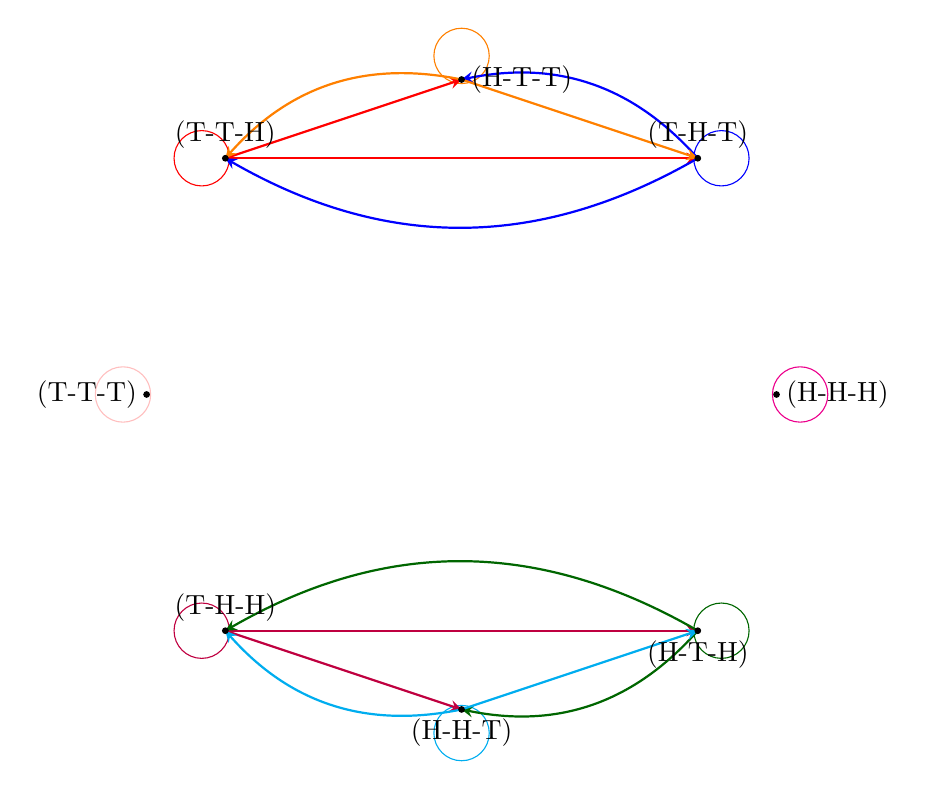
\begin{tikzpicture}[arrow/.style = {thick,-stealth}]
                \solution{
                    % loops
                    \draw[red]              (-3.3,    3)    circle (10pt);
                    \draw[blue]             (3.3,     3)    circle (10pt);
                    \draw[orange]           (0,     4.3)    circle (10pt);
                    \draw[purple]           (-3.3,    -3)   circle (10pt);
                    \draw[black!60!green]   (3.3,     -3)   circle (10pt);
                    \draw[cyan]             (0,     -4.3)   circle (10pt);
                    \draw[pink]             (-4.3,    0)    circle (10pt);
                    \draw[magenta]          (4.3,     0)    circle (10pt);
                }{}

                \solution{
                    % 1 point each
                    \draw[arrow,red] (-3,3) to (3,3);
                    \draw[arrow,red] (-3,3) to (0,4);
                    
                    \draw[arrow,blue] (3,3)  to[bend left] (-3,3);
                    \draw[arrow,blue] (3,3)  to[bend right] (0,4);
                    
                    \draw[arrow,orange] (0,4) to[bend right] (-3,3);
                    \draw[arrow,orange] (0,4) to (3,3);
                }{}
                \filldraw (-3,3)    circle (1pt) node[above] { (T-T-H) };   % 1
                \filldraw (3,3)     circle (1pt) node[above] { (T-H-T) };   % 1
                \filldraw (0,4)     circle (1pt) node[right] { (H-T-T) };   % 1

                \solution{
                    % 2 points each
                    \draw[arrow,purple] (-3,-3) to (3,-3);
                    \draw[arrow,purple] (-3,-3) to (0,-4);

                    \draw[arrow,black!60!green] (3,-3) to[bend right] (-3,-3);
                    \draw[arrow,black!60!green] (3,-3) to[bend left] (0,-4);

                    \draw[arrow,cyan] (0,-4) to[bend left] (-3,-3);
                    \draw[arrow,cyan] (0,-4) to (3,-3);
                }{}
                \filldraw (-3,-3)   circle (1pt) node[above] { (T-H-H) };   % 2
                \filldraw (3,-3)    circle (1pt) node[below] { (H-T-H) };   % 2
                \filldraw (0,-4)    circle (1pt) node[below] { (H-H-T) };   % 2
                
                \filldraw (-4,0)    circle (1pt) node[left]  { (T-T-T) };   % 0
                \filldraw (4,0)     circle (1pt) node[right] { (H-H-H) };   % 3
            \end{tikzpicture}
        \end{center}
        
    \end{questionNOGRADE}
       
\notonkey{ \newpage }{ \hrulefill }

    \begin{intro}{Symmetry}
        A relation $R$ on a set $A$ is said to be symmetric if, for all $a,b \in A$, if $(a,b) \in R$, then $(b,a) \in R$.

        ~\\ In terms of arrow diagrams, a symmetric relation has the property that every pair of nodes connected by an arrow is actually connected by two arrows, one in each direction.
        \footnote{Discrete Mathematics, Ensley and Crawley}
    \end{intro}

    % -------------------------------------------------------------%
    % - QUESTION --------------------------------------------------%
    % -------------------------------------------------------------%
    \stepcounter{question}
    \begin{questionNOGRADE}{\thequestion}

        For each of the following relations given, decide if the relation is symmetric. If not, give an example to illustrate this.

        \begin{itemize}
            \item[a.]   $R_{1} = \{ (a, b) \in \mathbb{Z} \times \mathbb{Z} : a + b$ is even $\}$.
                        \\ \\  If $a+b$ is even, then is $b+a$ also even?

                        \solution{ yes }{ \vspace{4cm} }

            \item[b.]   $R_{2} = \{ (a,b) \in \mathbb{Z} \times \mathbb{Z} : a + 2b$ is even $\}$.
                        \\ \\ For two numbers $(a,b)$, if $a+2b$ is even, then is $(b,a)$ (or $b + 2a$) also even?

                        \solution{ no. Example: (4,2) vs. (2,4), and (2,1) vs. (1,2). }{ \vspace{2cm} }
        \end{itemize}
    \end{questionNOGRADE}

\notonkey{ \newpage }{ \hrulefill }
 
    \begin{intro}{Review: Properties of a relation}
        Let $R$ be a binary relation on set $A$.

        \subparagraph{Reflexive:} $R$ is said to be reflexive if
        $(a,a) \in R$ for all $a \in A$. In terms of the arrow
        diagram, this means that \textbf{every node has a loop}.

        \subparagraph{Irreflexive:} A relation $R$ on set $A$ is irreflexive
        if, for all $a \in A$, $(a,a) \not\in R$. On the arrow diagram,
        this means \textbf{there are no loops.}

        \begin{center}
            \begin{tabular}{p{5cm} p{4cm} p{4cm}}
                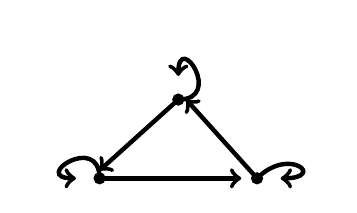
\begin{tikzpicture}[arrow/.style = {thick,-stealth}]
                    \draw[->,ultra thick] (0,0) -- (1.8,0);
                    \draw[->,ultra thick] (2,0) -- (1.1,1);
                    \draw[->,ultra thick] (1,1) -- (0,0.1);
                    
                    \draw[->,ultra thick] (0,0) to [out=90, in=180, looseness=5] (-0.3,0);
                    \draw[->,ultra thick] (2,0) to [out=45, in=0, looseness=5] (2.3,0);
                    \draw[->,ultra thick] (1,1) to [out=0, in=90, looseness=5] (1,1.3);
                    
                    \filldraw (0,0) circle (2pt);
                    \filldraw (2,0) circle (2pt);
                    \filldraw (1,1) circle (2pt);
                \end{tikzpicture}
                &
                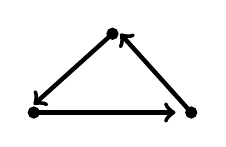
\begin{tikzpicture}[arrow/.style = {thick,-stealth}]
                    \draw[->,ultra thick] (0,0) -- (1.8,0);
                    \draw[->,ultra thick] (2,0) -- (1.1,1);
                    \draw[->,ultra thick] (1,1) -- (0,0.1);
                    
                    \filldraw (0,0) circle (2pt);
                    \filldraw (2,0) circle (2pt);
                    \filldraw (1,1) circle (2pt);
                \end{tikzpicture}
                &
                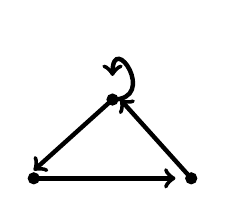
\begin{tikzpicture}[arrow/.style = {thick,-stealth}]
                    \draw[->,ultra thick] (0,0) -- (1.8,0);
                    \draw[->,ultra thick] (2,0) -- (1.1,1);
                    \draw[->,ultra thick] (1,1) -- (0,0.1);
                    \draw[->,ultra thick] (1,1) to [out=0, in=90, looseness=5] (1,1.3);
                    
                    \filldraw (0,0) circle (2pt);
                    \filldraw (2,0) circle (2pt);
                    \filldraw (1,1) circle (2pt);
                \end{tikzpicture}

                \\
                \tab Reflexive &  Irreflexive &  \tab[0.5cm]Neither
            \end{tabular}
        \end{center}

        \subparagraph{Symmetric:} $R$ is called symmetric if
        for all $a,b \in A$, if $a \neq b$ and $(a,b) \in R$,
        then $(b,a) \in R$. In terms of the arrow diagram, this
        means that \textbf{every arrow goes in both directions}.

        \subparagraph{Antisymmetric:} $R$ is called antisymmetric if
        for all $a,b \in A$, if $a \neq b$ and $(a,b) \in R$,
        then $(b,a) \not\in R$. In terms of the arrow diagram, this
        means that \textbf{arrows only go in one direction}.

        \begin{center}
            \begin{tabular}{p{5cm} p{4cm} p{4cm}}
                \tab
                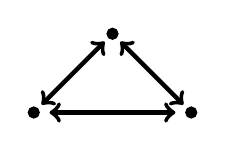
\begin{tikzpicture}[arrow/.style = {thick,-stealth}]
                    \draw[<->,ultra thick] (0.2,0) -- (1.8,0);
                    \draw[<->,ultra thick] (1.9,0.1) -- (1.1,0.9);
                    \draw[<->,ultra thick] (0.9,0.9) -- (0.1,0.1);
                    
                    \filldraw (0,0) circle (2pt);
                    \filldraw (2,0) circle (2pt);
                    \filldraw (1,1) circle (2pt);
                \end{tikzpicture}
                &
                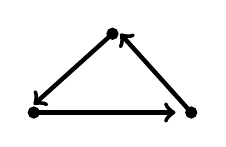
\begin{tikzpicture}[arrow/.style = {thick,-stealth}]
                    \draw[->,ultra thick] (0,0) -- (1.8,0);
                    \draw[->,ultra thick] (2,0) -- (1.1,1);
                    \draw[->,ultra thick] (1,1) -- (0,0.1);
                    
                    \filldraw (0,0) circle (2pt);
                    \filldraw (2,0) circle (2pt);
                    \filldraw (1,1) circle (2pt);
                \end{tikzpicture}
                &
                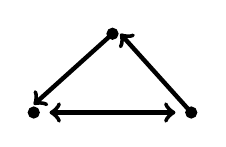
\begin{tikzpicture}[arrow/.style = {thick,-stealth}]
                    \draw[<->,ultra thick] (0.2,0) -- (1.8,0);
                    \draw[->,ultra thick] (2,0) -- (1.1,1);
                    \draw[->,ultra thick] (1,1) -- (0,0.1);
                    
                    \filldraw (0,0) circle (2pt);
                    \filldraw (2,0) circle (2pt);
                    \filldraw (1,1) circle (2pt);
                \end{tikzpicture}

                \\
                \tab Symmetric &  Antisymmetric &  \tab[0.5cm]Neither
            \end{tabular}
        \end{center}
        
        \subparagraph{Transitive:} $R$ is transitive if, whenever
        $(a,b) \in R$ and $(b,c) \in R$, it must also be the case
        that $(a,c) \in R$. In terms of the arrow diagram, this
        means that \textbf{whenever you can follow two arrows
        to get from node $a$ to node $c$, you can also get there
        along a single arrow}.
        \footnote{Discrete Mathematics, Ensley and Crawley}
    \end{intro}
    
\notonkey{ \newpage }{ \hrulefill }

    % -------------------------------------------------------------%
    % - QUESTION --------------------------------------------------%
    % -------------------------------------------------------------%
    \stepcounter{question}
    \begin{questionNOGRADE}{\thequestion}

        Let $S = \{1, 2, 3\}$. For each of the following relations on $\wp(S)$,
        draw the arrow diagram identify its properties: Reflexive,
        Transitive, and/or Symmetric.

        ~\\
        a. $R_{1} = \{ (A,B) \in \wp(S) \times \wp(S) : A \subseteq B \}$ \\
        Hint: Two sets $A$ and $B$ are ``equivalent'' if $A$ is a subset (or equal to) $B$.
        The empty set is considered a subset of everything.

        \solution{
            It is reflexive and transitive, but not symmetric. \\ Example:
            (\{1\}, \{1,2\}) $\in$ $R_{1}$ but (\{1,2\}, \{1\}) is not.
            (This is antisymmetric.)
        }{
            \Square\ Is reflexive   \tab    \Square\ Is symmetric   \tab    \Square\ Is transitive
        }

        \begin{center}
            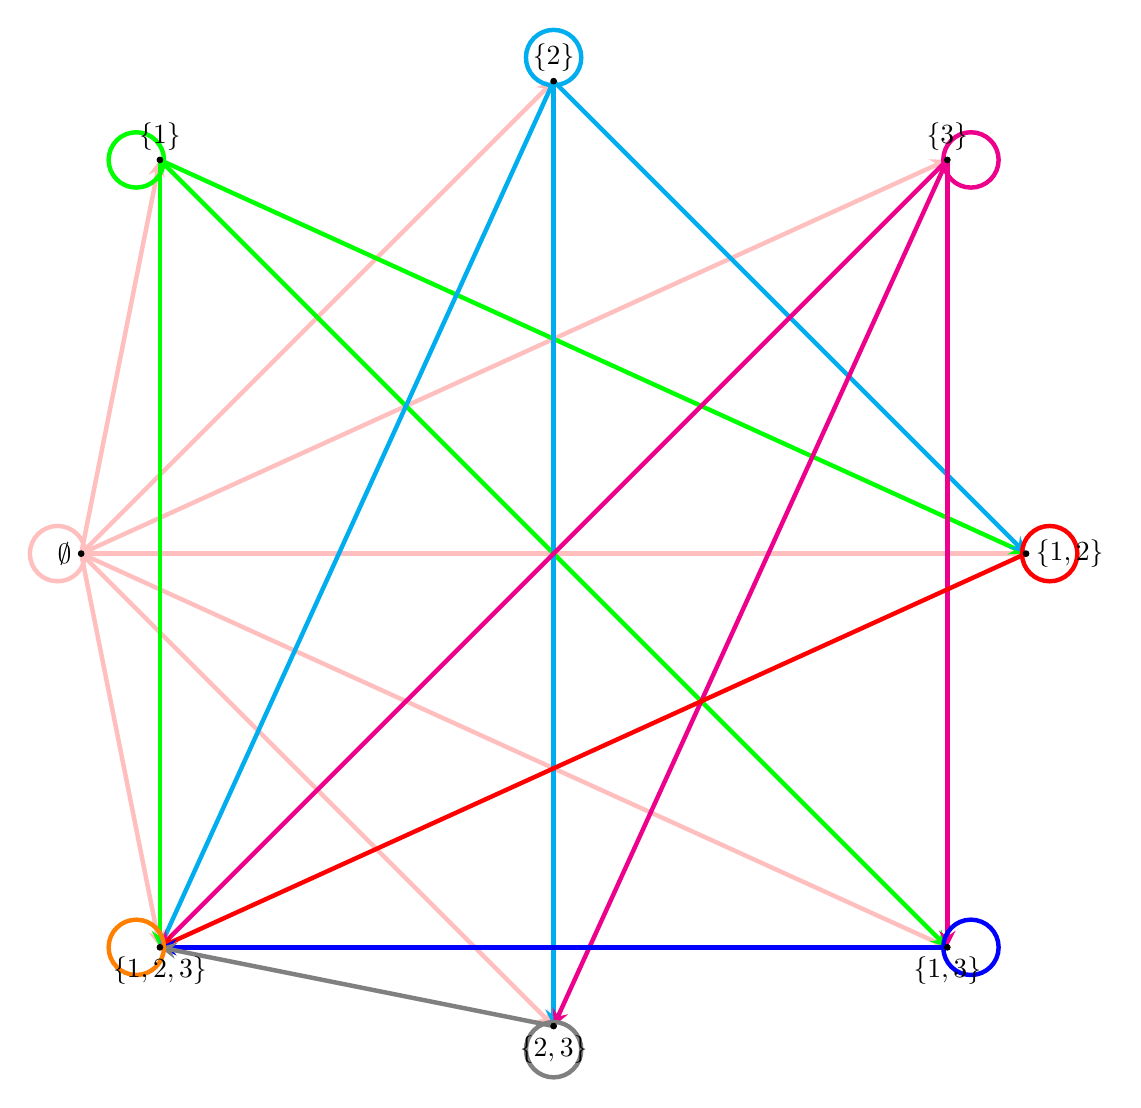
\begin{tikzpicture}[arrow/.style = {ultra thick,-stealth}]
                \solution{
                    \draw[arrow,pink] (-6,0) -- (-5,5);
                    \draw[arrow,pink] (-6,0) -- (0,6);
                    \draw[arrow,pink] (-6,0) -- (5,5);
                    \draw[arrow,pink] (-6,0) -- (6,0);
                    \draw[arrow,pink] (-6,0) -- (5,-5);
                    \draw[arrow,pink] (-6,0) -- (0,-6);
                    \draw[arrow,pink] (-6,0) -- (-5,-5);
                    \draw[pink,ultra thick] (-6.3,0) circle (10pt);

                    \draw[arrow,green] (-5,5) to (-5,-5);
                    \draw[arrow,green] (-5,5) to (6,0);
                    \draw[arrow,green] (-5,5) to (5,-5);
                    %\draw[arrow,green] (-5,5) to (0,-6); % Error
                    \draw[green,ultra thick] (-5.3,5) circle (10pt);

                    \draw[arrow,cyan] (0,6) to (-5,-5);
                    \draw[arrow,cyan] (0,6) to (6,0);
                    \draw[arrow,cyan] (0,6) to (0,-6);
                    \draw[cyan,ultra thick] (0,6.3) circle (10pt);

                    \draw[arrow,magenta] (5,5) to (-5,-5);
                    \draw[arrow,magenta] (5,5) to (5,-5);
                    \draw[arrow,magenta] (5,5) to (0,-6);
                    \draw[magenta,ultra thick] (5.3,5) circle (10pt);

                    \draw[arrow,red] (6,0) to (-5,-5);
                    \draw[red,ultra thick] (6.3,0) circle (10pt);

                    \draw[arrow,blue] (5,-5) to (-5,-5);
                    \draw[blue,ultra thick] (5.3,-5) circle (10pt);

                    \draw[arrow,gray] (0,-6) to (-5,-5);
                    \draw[gray,ultra thick] (0,-6.3) circle (10pt);

                    \draw[orange,ultra thick] (-5.3, -5) circle (10pt);
                }{}

                \filldraw (-6,0)        circle (1pt) node[left]  { $\emptyset$ };
                \filldraw (-5,5)        circle (1pt) node[above] { $\{1\}$ };
                \filldraw (0,6)         circle (1pt) node[above] { $\{2\}$ };
                \filldraw (5,5)         circle (1pt) node[above] { $\{3\}$ };
                \filldraw (6,0)         circle (1pt) node[right] { $\{1,2\}$ };
                \filldraw (5,-5)        circle (1pt) node[below] { $\{1,3\}$ };
                \filldraw (0,-6)        circle (1pt) node[below] { $\{2,3\}$ };
                \filldraw (-5,-5)       circle (1pt) node[below] { $\{1,2,3\}$ };
            \end{tikzpicture}
        \end{center}
        
\newpage

        ~\\
        b. $R_{2} = \{ (A,B) \in \wp(S) \times \wp(S) : A \cap B = \emptyset \}$ \\
        Hint: Two sets $A$ and $B$ are ``equivalent'' if they have nothing in common.
        The empty set is also considered to not have anything in common with any other
        set, including itself.
        
        \solution{ It is symmetric but not reflexive: (\{1\}, \{1\}) $\not\in R$,
        and not transitive: (\{1\},\{3\}) $\in R$, but (\{1\}, \{1\}) $\not\in R$. }
        {
            \Square\ Is reflexive   \tab    \Square\ Is symmetric   \tab    \Square\ Is transitive
        }

        \begin{center}
            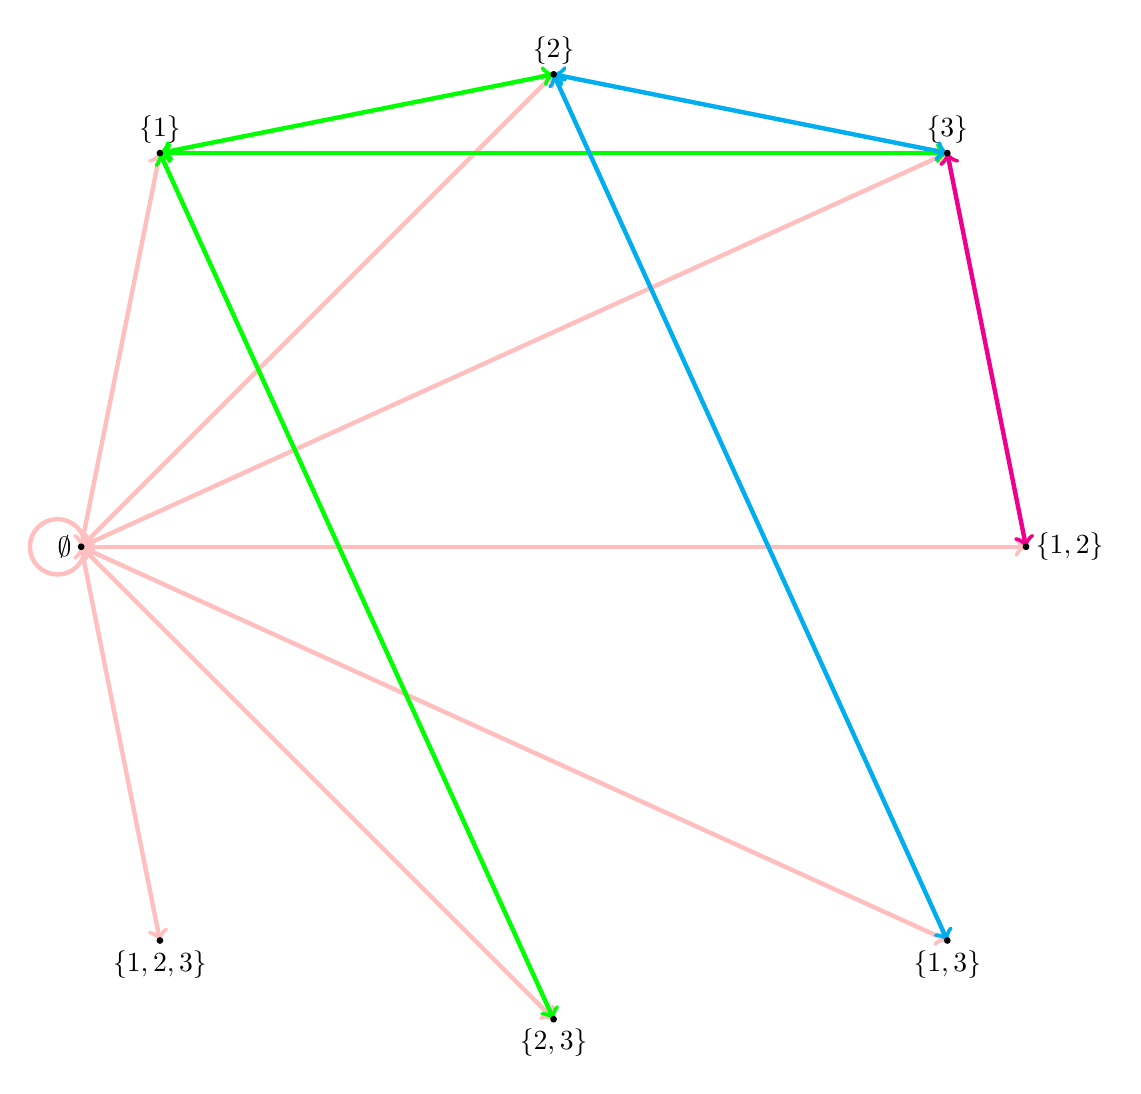
\begin{tikzpicture}
                \solution{
                    \draw[pink,ultra thick] (-6.3,0) circle (10pt);
                    \draw[pink,<->,ultra thick] (-6,0) to (-5,5);
                    \draw[pink,<->,ultra thick] (-6,0) to (0,6);
                    \draw[pink,<->,ultra thick] (-6,0) to (5,5);
                    \draw[pink,<->,ultra thick] (-6,0) to (6,0);
                    \draw[pink,<->,ultra thick] (-6,0) to (5,-5);
                    \draw[pink,<->,ultra thick] (-6,0) to (0,-6);
                    \draw[pink,<->,ultra thick] (-6,0) to (-5,-5);

                    \draw[green,<->,ultra thick] (-5,5) to (0,6);
                    \draw[green,<->,ultra thick] (-5,5) to (5,5);
                    \draw[green,<->,ultra thick] (-5,5) to (0,-6);

                    \draw[cyan,<->,ultra thick] (0,6) to (5,5);
                    \draw[cyan,<->,ultra thick] (0,6) to (5,-5);

                    \draw[magenta,<->,ultra thick] (5,5) to (6,0);
                }{}

                \filldraw (-6,0)        circle (1pt) node[left]  { $\emptyset$ };
                \filldraw (-5,5)        circle (1pt) node[above] { $\{1\}$ };
                \filldraw (0,6)         circle (1pt) node[above] { $\{2\}$ };
                \filldraw (5,5)         circle (1pt) node[above] { $\{3\}$ };
                \filldraw (6,0)         circle (1pt) node[right] { $\{1,2\}$ };
                \filldraw (5,-5)        circle (1pt) node[below] { $\{1,3\}$ };
                \filldraw (0,-6)        circle (1pt) node[below] { $\{2,3\}$ };
                \filldraw (-5,-5)       circle (1pt) node[below] { $\{1,2,3\}$ };
            \end{tikzpicture}
        \end{center}
        
\newpage

        ~\\
        c. $R_{3} = \{ (A,B) \in \wp(S) \times \wp(S) : n(A) = n(B) \}$ \\
        Hint: Two sets $A$ and $B$ are ``equivalent'' if they have the same amount of elements.
        
        \solution{
            It is reflexive, symmetric, and transitive.
        }{
            \Square\ Is reflexive   \tab    \Square\ Is symmetric   \tab    \Square\ Is transitive
        }

        \begin{center}
            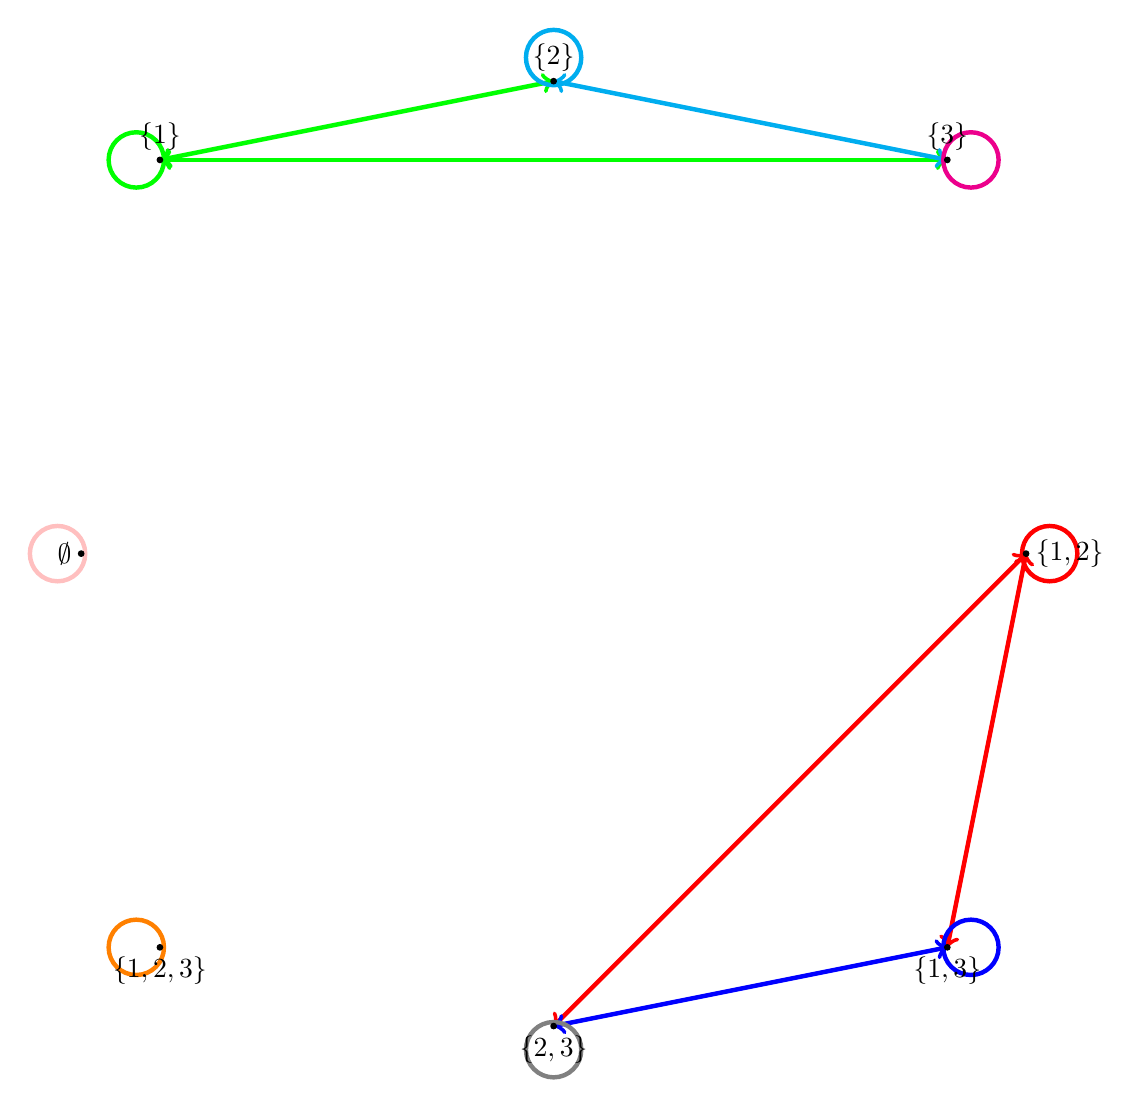
\begin{tikzpicture}[arrow/.style = {thick,-stealth}]
                \solution{
                    \draw[pink,ultra thick] (-6.3,0) circle (10pt);
                    
                    \draw[green,ultra thick] (-5.3,5) circle (10pt);
                    \draw[green,ultra thick,<->] (-5,5) to (0,6);
                    \draw[green,ultra thick,<->] (-5,5) to (5,5);
                    
                    \draw[cyan,ultra thick] (0,6.3) circle (10pt);
                    \draw[cyan,ultra thick,<->] (0,6) to (5,5);
                    
                    \draw[magenta,ultra thick] (5.3,5) circle (10pt);
                    
                    \draw[red,ultra thick] (6.3,0) circle (10pt);
                    \draw[red,ultra thick,<->] (6,0) to (5,-5);
                    \draw[red,ultra thick,<->] (6,0) to (0,-6);
                    
                    \draw[blue,ultra thick] (5.3,-5) circle (10pt);
                    \draw[blue,ultra thick,<->] (5,-5) to (0,-6);
                    
                    \draw[gray,ultra thick] (0,-6.3) circle (10pt);
                    
                    \draw[orange,ultra thick] (-5.3, -5) circle (10pt);
                }{}

                \filldraw (-6,0)        circle (1pt) node[left]  { $\emptyset$ };
                \filldraw (-5,5)        circle (1pt) node[above] { $\{1\}$ };
                \filldraw (0,6)         circle (1pt) node[above] { $\{2\}$ };
                \filldraw (5,5)         circle (1pt) node[above] { $\{3\}$ };
                \filldraw (6,0)         circle (1pt) node[right] { $\{1,2\}$ };
                \filldraw (5,-5)        circle (1pt) node[below] { $\{1,3\}$ };
                \filldraw (0,-6)        circle (1pt) node[below] { $\{2,3\}$ };
                \filldraw (-5,-5)       circle (1pt) node[below] { $\{1,2,3\}$ };
            \end{tikzpicture}
        \end{center}
    \end{questionNOGRADE}

\end{document}







